\documentclass[tikz]{standalone}
\usepackage{tikz}
\usetikzlibrary{positioning, graphs}
\usetikzlibrary{graphs.standard}
\begin{document}
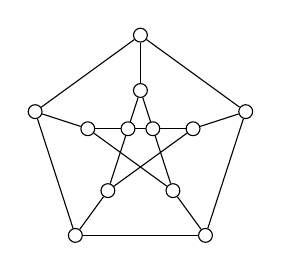
\begin{tikzpicture}
		[every node/.style={draw, circle,inner sep = 0em, minimum size = 0.5em}]
		\graph[clockwise, radius = 4em, empty nodes]{subgraph C_n[n = 5, name = A]};
		\graph[clockwise, radius = 2em, empty nodes] {subgraph I_n [n = 5, name = B]};
		
		\foreach \i [evaluate={\j=int(mod(\i+2,5)+1);}] in {1,...,5}{ \draw (A \i) -- (B \i); }
		
		\draw[-] (B 1) to (B 3);
		\draw[-] (B 2) to (B 4);
		\draw[-] (B 3) to (B 5);
		\draw[-] (B 4) to (B 1);
		\draw[-] (B 5) to (B 2);
		
		\node[fill=white] (a) at (intersection of B 1--B 3 and B 5--B 2) {};
		\node[fill=white] (b) at (intersection of B 4--B 1 and B 5--B 2) {};
\end{tikzpicture}
\end{document}